% !Mode:: "TeX:UTF-8"
%%==========================
%% chapter01.tex for SJTU Master Thesis
%% based on CASthesis
%% modified by wei.jianwen@gmail.com
%% version: 0.3a
%% Encoding: UTF-8
%% last update: Dec 5th, 2010
%%==================================================

%\bibliographystyle{sjtu2} %[此处用于每章都生产参考文献]
\chapter{引言}
\label{chap:intro}

\section{背景和意义}
人体工程学是计算机视觉领域的核心内容,它可以影响到人们方方面面的生活。
例如人脸识别在安全领域的应用,衣服属性分析在衣服搜索领域的应用等等。
这些技术中最基础之一是人体姿势预测。
一般来说,人体姿势预测(HPE)可以应用到很多领域,比如动作识别、图像分割等等。
然而它是一个非常困难的问题,特别是在没有任何辅助信息的情况下,而且对于手臂和腿部等变化比较丰富的人体部位。

众所周知,可以用上下文信息(比如衣服属性、边缘信息等)来解决这个难题。
在图1中,a,b,c是三个候选结果,很明显如果我们知道一些上下文信息,很容易判断出只有c是正确解。
因此,这种方法叫做上下文模型,即就是将图片上已知的信息加入到HPE问题中,来提高模型的准确性。
近来年,有很多学者做了这方面的工作\cite{deeppose,cvpr09}, 比如\cite{deeppose},他将前背景和后背景对比信息加入到人体姿势预测中。
Ladicky\cite{cvpr09}等人将人体姿势预测与图像分割联系起来,用通过这种联合学习的方式提高HPE的精度。
在Jie Shen\cite{shen2014unified}等人的工作中,他们将人体姿势和衣服属性联合起来进行求解\cite{cvpr09}。

\section{研究内容和方法}
虽然已有的很多工作利用上下文信息提高了人体姿势预测的精度,但是他们都需要进行大量的上下文信息标注才能进行训练,这个非常耗时而且不太实际,对于大数据来说。
在本文中,我们提出了基于隐式衣服属性的人体姿势预测。
我们通过对图画式结构进行扩展来形式化人体姿势预测问题,特别地,我们将衣服属性作为隐变量来建模。
跟传统的基于标注信息进行预测的方法不同,我们不需要显示的标注额外的信息,而且可以高效的进行求解。
在本文中,我们定义了几种比较重要的衣服属性,并且建立了衣服属性和人体部位之间的关系(比如袖子和手臂等)。
进而,我们设计了两种特征,一是人体躯干对应的特征,二是人体躯干和衣服属性的联合特征。
我们采用隐式结构式支持向量机算法来进行模型的训练。
所有的隐变量问题都会涉及到隐变量的初始化问题,我们采用K-Means聚类算法来初始化隐变量。
接着,我们采用增量迭代的方式来进行参数的学习,即就是最小化隐式结构式支持向量机的目标函数。
更为详尽的,我们采用迭代的方式来训练模型,首先当衣服属性变量确定的时候,我们采用动态规划的算法进行人体姿势的求解。
另一步是,当人体姿势确定的时候,我们可以采用第三章提出的算法来确定衣服属性的变量。
在两个公开的数据集上,我们进行了有力的实验,结果显示我们的方法超过了传统最好的方法,并且我们将具有同样衣服属性的照片聚在了一起。

\section{本文的贡献}
总体来说,本文有三大主要贡献:

(1)\textbf{我们提出了一个隐式衣服属性的方法,可以隐性的将衣服属性加入到人体姿势预测问题中。}
通过上述讨论可知,姿势估计和衣服属性识别这两个问题之间有很强的关联性,但是之前的工作,
无论是直接利用姿势估计来进行服饰分析,还是迭代地分割服饰再优化姿势,
或是定义一些能量函数然后通过参数来平衡姿势和服饰的权重,都没有很好地在一个框架下对这两个问题进行统一的建模求解。
在我们的工作中,考虑衣服属性的作用,并且将它作为一个隐式变量,这样就不用手动的去标注衣服属性。

(2)\textbf{我们定义了一些有效的特征来描述人体部位和衣服属性之间的关系。}
特征是用来刻画问题输入对象的重要参数,所以特征的设计选择直接影响着后续的问题建模与求解。 特征设计是机器学习领域非常重要的问题之一,往往一个问题的特征设计好坏与否直接关系到问题求解的优劣。
在我们工作中,人体肢干相关的特征,我们主要考虑两个方面,一是肢干本身的特征,二是相邻肢干的联合特征。 HOG特征在前人的很多工作中得到应用,它被证明可以很好的描述物体的形状,因而在我们的工作中,肢干本身的特征采用HOG特征。 关于相邻肢干的联合特征,我们主要考虑两个肢干的相对位置、相对角度和相对距离。


(3)\textbf{我们提出了一个高效的算法来解决有环图的预测问题(这是一个极其有难度的问题)。}
在以往的工作中,大家对于分别求解两个问题时,都假定问题满足树结构,这样可以使得求解非常高效。 但是现在我们对于两个问题同时建模,破坏了树结构的假设,为此,我们提出了一种迭代求解的算法, 在每一次的迭代过程中,人体的姿势或者衣服的属性都是固定的,从而问题可以规约成一个树模型的求解过程, 使得每一轮的求解可以使用动态规划法进行高效的求解。

\begin{figure}[tbp]
    \centering
    \subfigure[]{
        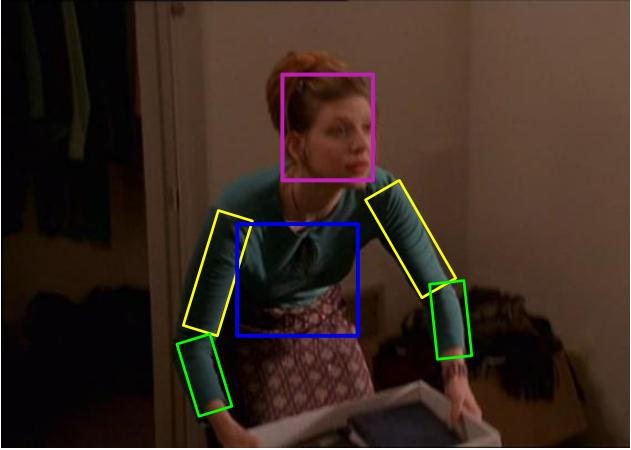
\includegraphics[width=.3\textwidth]{img/eg_a.pdf}
    }
    \subfigure[]{
        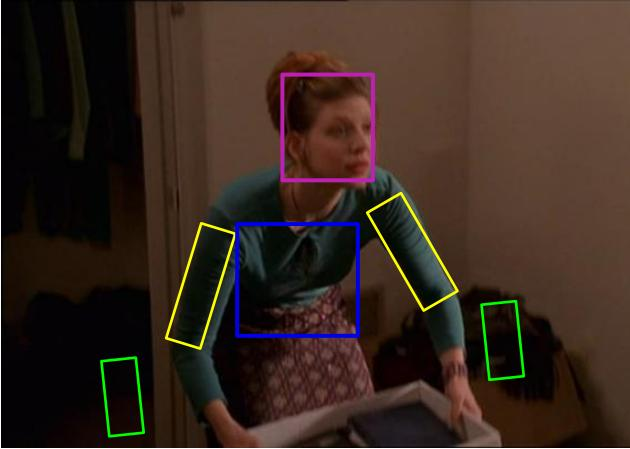
\includegraphics[width=.3\textwidth]{img/eg_b.pdf}
    }
    \subfigure[]{
        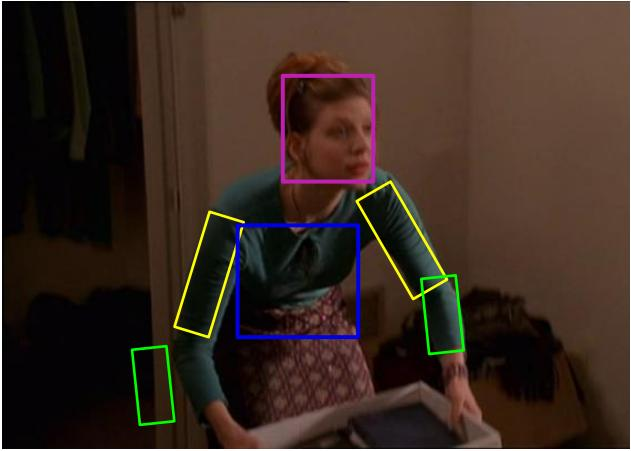
\includegraphics[width=.3\textwidth]{img/eg_c.pdf}
    }
    \caption{
    \textbf{在人体姿势预测问题中加入衣服属性的动机}
图中所示的三个人体姿势预测的结果,图(b)和图(c)中除了下臂预测错误,其它躯干预测的结果都是正确的。
对于图(c)来说,我们可以通过形状特征来得出左右手臂的不同之处,从而可以将(c)排除掉,
但是在图(b)中,左右手臂的不同之处很微小,我们很难用形状特征来区分出左右手臂。
如果我们知道图中衣服属性的类别值,比如袖子的类别和颜色等。
这样我们就可以根据袖子的颜色或者类别值来区分左右手臂,因为图(b)中左右手臂对应的衣服属性袖子颜色不一致。
最后,我们得到了正确的预测结果,即图(a)。
    }
    \label{fig:eg}
\end{figure}


\section{论文组织}
接下来我们将逐章来介绍我们的工作。
在第二章中,我们介绍了相关的工作,主要分为人体姿势预测(Human Pose Estimation)、衣服属性分析(Clothing Attribute Analysis)、隐变量结构式学习(Structure Learning with Latent Variables)等特定问题领域来介绍。
在第三章中,我们会介绍本文工作的问题背景,主要对本文中涉及到的技术做一个很好的概括。
主要分为图模型(Graphic Model)、图画式结构(Pictorial Structure)、结构式学习(Structure Learning)、形变部位模型(Deformable Part Model)等知识领域来介绍。
在第四章中,我们主要介绍了我们提出的模型和算法,主要分为联合特征设计、模型训练、姿势预测算法等部分来介绍。
第五章我们节选了部分之前跟人体姿势相关的工作来讲述,主要包括基于多媒体数据的事件挖掘(Event Detection)、基于电商平台的衣服搜索(Clothing Search)、基于图片的广告推荐(Advertisement Recommendation)等。
主要阐述人体姿势预测在这些问题上的应用。
在第六章中,我们介绍了实验部分,对数据集、评测指标、实验结果等进行了详细的介绍。
第七章,我们进行了总结,并对未来的工作进行了展望。

\section{本章小结}
本章中,我们简要的介绍了前人在人体姿势识别方面的工作,以及他们的不足,从而提出我们的方法,
克服前人工作的不足支持。
并且我们通过例子说明了加入衣服属性的良好效果。
